% Author: Joshua Carey

%
\let\textcircled=\pgftextcircled
\chapter{Methodology}
\label{chap:aims_and_opjectives}

\initial{T}his section will investigate the approach taken to create an autonomous kite-powered vessel.
- We need a physics engine
-we need to model a boat so that it behaves with realistic movements
- need to be able to run machine learning in the physics simulations

\initial{T}he future of autonomous navigation in maritime settings is not limited to large vessels plying the world's oceans; smaller, nimble crafts, harnessing natural forces such as wind, present their own set of challenges and opportunities. Imagine a vessel, propelled not just by the currents below, but by the gusts above, using a kite to harness the power of the wind. This not only promises sustainable navigation but also offers a glimpse into the intricate dance between machine intelligence, physics, and nature's unpredictability. This project dives deep into simulating such a system— a kite-powered boat that autonomously navigates its environment. This methodology section elucidates the steps taken to bridge the gap between vision and virtual reality.

\section{A Simulation Environment}
For any machine learning endeavor, especially one with such intricate physical dynamics, the choice of simulation environment is paramount. Not only does it provide the playground for our AI agent to learn and make mistakes safely, but it also serves as a litmus test for the robustness and realism of the designed model.

Given the myriad of choices available, the Unity game engine emerged as the most suitable platform. Beyond its reputation in gaming, Unity is recognized for its potent physics engine, an essential feature for our project. The inherent support for mesh bodies, colliders, and a variety of joints made it an attractive option for simulating the kite-boat system, a complex dance of forces, and counterforces.

\subsection{Water Dynamics}
Central to our simulation is the depiction of water, the medium in which our boat will navigate. Here, the Unity HDRP Water System 16.0.3 [cite] came to our aid. Bundled with Unity 2023.2.0b9 [cite], this water system provides a realistic representation of water with its undulating waves, refractions, and reflections. The first challenge, therefore, was to design a boat that could navigate this dynamic surface.

\subsection{Buoyancy}
Buoyancy, the force that allows ships to float, was the first physical property to be addressed. Rooted in Archimedes' Principle, it dictates that the buoyant force exerted on a submerged body is equivalent to the weight of the fluid displaced by that body. In our Unity environment, the boat's hull, represented as a 'mesh' with an associated 'mesh collider', was divided into myriad small triangles or Voxels. These Voxels became the fundamental units for calculating buoyancy, allowing for a granular and realistic representation of the boat's interaction with water.

\subsection{Rudder Dynamics}
While buoyancy ensures our boat doesn't sink, it's the rudder that grants it direction. Modeled as a rigid body in Unity, the rudder was designed as a symmetric foil, with
\subsection{Buoyancy}
To model buoyancy accurately, first the maths had to be reviewed. When a body is submerged in a fluid the fluid exerts a force on the surface of the body, due to the pressure in the fluid. Archimedes Principal states that "The upward buoyant force that is exerted on a body immersed in a fluid, whether partially or fully submerged, is equal to the weight of the fluid that the body displaces and acts in the upward direction at the center of mass of the displaced fluid", shown in equation \ref{archimedes}. In order to model the buoyancy of a complex object, such as a boat hull, the 'amount' of boat below the water needed to be calculated. In Unity the boat hull was a 'mesh' with a 'mesh collider' attached to it, this was incredibly helpful as it takes on the complex challenge of splitting the surface of the hull into many small triangles or Voxels 


\begin{equation}
    F_B = \rho_{w}gV
    \label{archimedes}
\end{equation}

The total Archimedes force (AF) of the entire boat was calculated using equation \ref{archimedes}, followed by a local AF at each Voxel. The water level, y component, was then computed at each voxel's (x,z) coordinates to determine if it was above or below the surface. If below the surface the component of the AF was applied vertically at each voxel. 

\subsection{Rudder}
The rudder was created as a rigid body and modeled as a simple symmetric foil using the force diagram in figure \ref{rudderForce}. The lift and drag forces were calculated using equations \ref{lift} and \ref{drag}, where ${C_l}$ is the lift coefficient, ${C_d}$ is the drag coefficient, A is the sing surface area, V is the velocity of the water and ${\rho}$ is the density of the water.



\begin{equation}
    L = {C_l}A\rho\frac{V^2}{2}
    \label{lift}
\end{equation}
\begin{equation}
    D = {C_d}A\rho\frac{V^2}{2}
    \label{drag}
\end{equation}
 
\begin{figure}
    \centering
    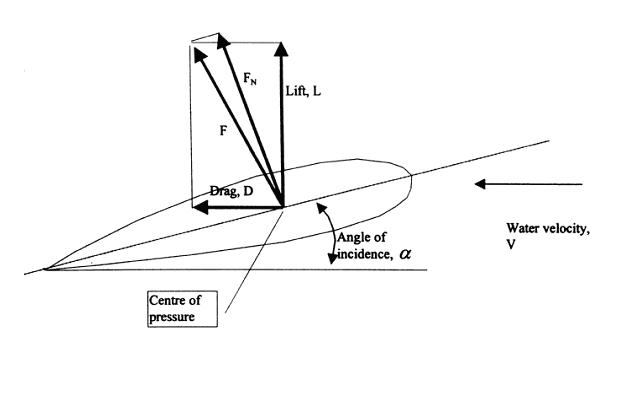
\includegraphics{chapters/chapter04/rudder.JPG}
    \caption{Force Diagram of a boat rudder}
    \label{rudderForce}
\end{figure}

\subsection{Course Generation}

\subsection{Mark Roundings}

\section{MLAgents}

\section{The Boat Agent}

\section{Initial Training}

\section{Optimization}

%=======
\label{sec:sec01}





%=========================================================